Software Development Life Cycle (SDLC) is a way to systematically approach software development.
It provides a methodology to improve quality of the desired product and the general work progress. 
Depending on the customer or end users and how clear the project's requirements are different approaches are needed. 
Among the different SDLC methods are the most common ones the older traditional ''Waterfall model'' and the newer ''Iterative model''. \cite{SDLC-Toolsqa}

This chapter will first briefly present the ''waterfall model'' and the ''iterative model'', And during these the argument for choosing the ''iterative model''.
Hereafter, the chapter will contain a description of each iteration throughout the project.


\section{Waterfall model}\label{sec:WaterfallModel}
The principle of the waterfall model,\cite{Waterfall-Toolsqa}, is that the software development process is divided into separate phases, which makes it a sequential design process.
Here the output, in form of documentation, of one phase serves as the input for the next one which means that no phase will start without the previous one being complete.
This is often illustrated as a downward going flow, see \cref{fig:Waterfall}, which is also the reason for its name.

\begin{figure}[H]
	\centering
	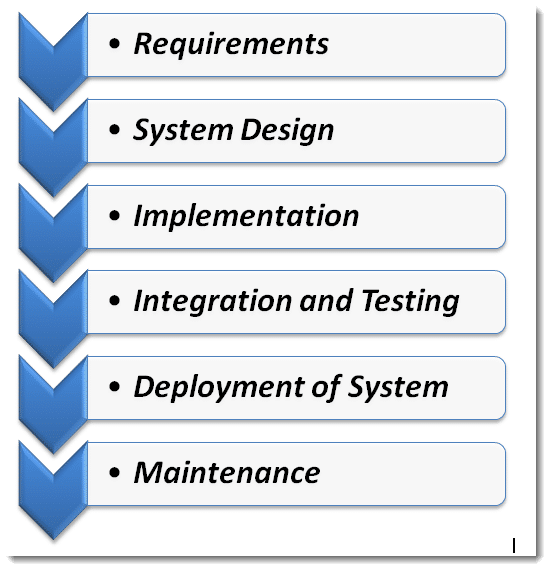
\includegraphics[width=0.4\textwidth]{billeder/WaterFall-Model.png}
	\caption{The Waterfall Model \cite{Waterfall-Toolsqa}.}\label{fig:Waterfall}
\end{figure}

\paragraph{The main benefits} of this model, is that it allows for departmentalization, which in theory makes it possible for separate teams to work at each phase without ever communicating with one another since only the documentation is necessary.
Another benefit of this system is how it is easy to manage since there are clear guidelines of what is needed before one phase is done and another can begin.

\paragraph{The main disadvantage} is on the other hand that because of this rigidity it becomes more difficult after every finished phase to go back and change things, when mistakes or misunderstandings of the concept has been made.
Therefore it is also not a beneficial model to use when there is a moderate to high risk that the requirements of the system changes.
%ville måske være bedre med en simpel textbf for at undgå ekstra mellemrum i pdfen
%Anna: Synes ikke selv det gør noget, kan god lide de to ting er skilt ad

Since the system developed in this project is done in cooperation with Ipsen, there is a moderate risk of the requirements changing.
This based on the risk of concept misunderstandings, since Ipsen is an expert in her field who has taken contact to software developers with no expertise in this field.
%ikke helt sikker på om jeg forstår this based delen af denne her sætning

\section{Iterative Model} \label{sec:iterativModel}
The main principle of the iterative model, \cite{Iterative-Toolsqa,InteractionDesign} is to divide the software development into a cycle of ''waterfalls'', it could also be seen as a form of ''multi-waterfalls'' model.
Instead of focusing on everything through every phase in the waterfall model, the development is done in pieces and at every iteration a little more is added to the product until it is finished.
Through each iteration the product and requirements are always being redetermined, redefined and further developed through the models activities and in collaboration with the client or users, until the final solution is reached.
Different iteration models are simplified versions of reality and are not meant to be prescriptive, and depending on the project it is not always possible to go through all of the phases described in these models. 
Three explicit models will be presented in the \cref{sec:Iterative1,sec:Iterative3}.


\paragraph{The main benefits}
of working iteratively is the continuous talk with the client and users which yields the opportunity to determine and redetermine what their needs truly are rather than just what they believe them to be.
This ongoing communication also makes it easier for catching mistakes and faulty software since only a little part is added at each iteration.
It is easier as well to clarify misconceptions of the products requirements \cref{sec:requirementsdefinition}.
The repeated correspondence with the client and users is likewise the center of the human-centered approach, mentioned in \cref{sec:PACT}, which is of great importance when designing and developing an interactive system.

\paragraph{The main disadvantage} of the iteration model is how adding functionality at every stage, may cause problems related to the system architecture since it had not been thought into the design to begin with, see \cref{sec:Bug}.
This may in worst case scenario cause for the whole system to be redesigned and re-implemented.
Another disadvantage with this model is also one of it strong suits and allures which is how it can become difficult to manage and keep track of the development, and when a iteration is done and a new one begin since it is ever changing.

% Henrik: Maaske ganske kort om hvordan vi har brugt den iterative model - bare et par linjer :-)
%Anna svar: Er det ikke det jeg har skrevet i 6.2.3? hvor jeg prøver kort at beskrive vores metode?

\subsection{The process of designing interaction systems}\label{sec:Iterative1}
In \cref{fig:DEBModel} it becomes apparent how it might be difficult to define when an iteration ends and a new one begins since it is possible to start at any point and to move back and forth between the activities as seen fit.
The four basic activities of this model are; \textit{understanding, design, envisionment} and \textit{evaluation}.

\begin{figure}[H]
	\centering
	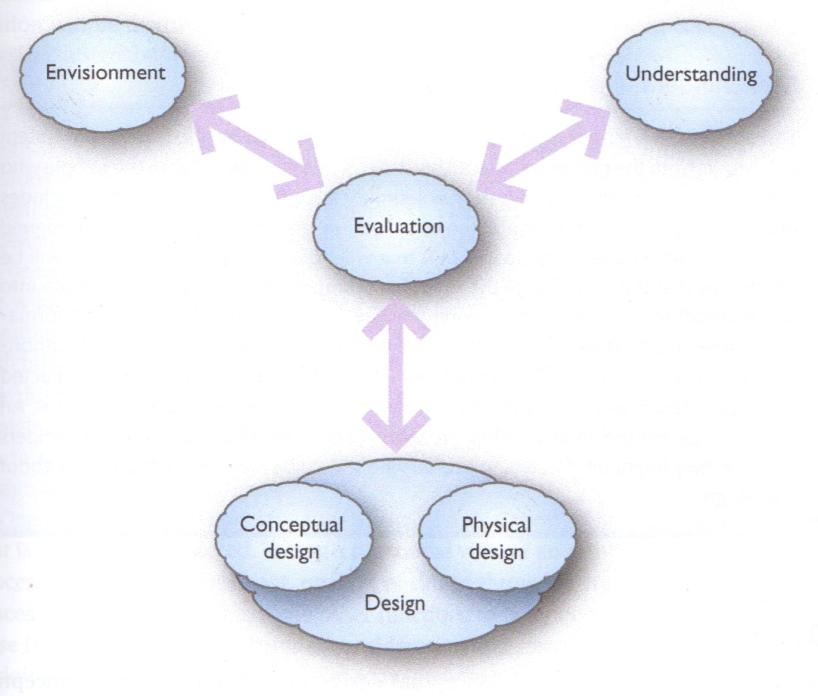
\includegraphics[width=0.5\textwidth]{billeder/DEBModel.jpg}
	\caption{Understanding, design, evaluation, envisionment \citep[p.~49]{Benyon}}\label{fig:DEBModel}
\end{figure}
'Understanding' is a broad term which covers among other establishing requirements, understanding the context of the developed system and the technological landscape.
%To be able to design a system with the user’s needs and wants in mind it is imperative to know the target users and which activities the system needs to support. 
The 'envisionment' activity concerns itself with determining appropriate media in which to render design ideas.
While the 'design' activity is done through conceptual- and physical design as seen in \cref{fig:DEBModel}.
These last two activities combines together to designing alternatives and prototyping.
'Evaluation' at the center of the model is where understandings and design ideas are confirmed or reevaluated with the client and/or users.
It is therefore a paramount activity since this is the catalyst for the human-centered development.

It is important to take note of as mentioned above, \cref{sec:iterativModel}, the model is a simplified version of reality.
It is therefore also possible to be using different phases in combination of each other at the same time, and it is therefore not strictly divided when working with the iterative model

\subsection{OOA\&D iteration model}\label{sec:Iterative3}
This section is based on Mathiassen, Munk-Madsen, Nielsen and Stage \cite{Rod-Aalborg}, unless anything else is stated.

In the OOA\&D method, \cite{Rod-Aalborg}, mentioned in \cref{sec:ClassEvent},  there are four basic activities; \textit{Problem-domain analysis, Application-domain analysis, Architectural design} and \textit{Component design}.
In between these activities  also lies programming and quality assurance.
The importance of each activity is relative in each iteration and the sequence changes from each development project.

%Anna: er det nødvendigt at skrive et afsnit om sammenligning af de fire aktiviteter?, da det i princippet er modeller til to forskellige ting tænker jeg ikke det er nødvendigt explicit at skrive ind her

In \cref{fig:SUModels} two different iterative models based on the OOA\&D method is shown.
The first model, \cref{fig:SUModel1} is a model closer to the traditional waterfall model though it is still an iterative process modeled.
The reason for it not to be a waterfall model is how the elements; architectural design, and programming, stretches across more phases.
The second model, \cref{fig:SUModel2} is on the other hand closer to the stereotype of a iterative model where each basic activity is done or at least considered in every iteration. 

\begin{figure}[H]
	\centering
	\begin{subfigure}[b]{0.48\textwidth}
		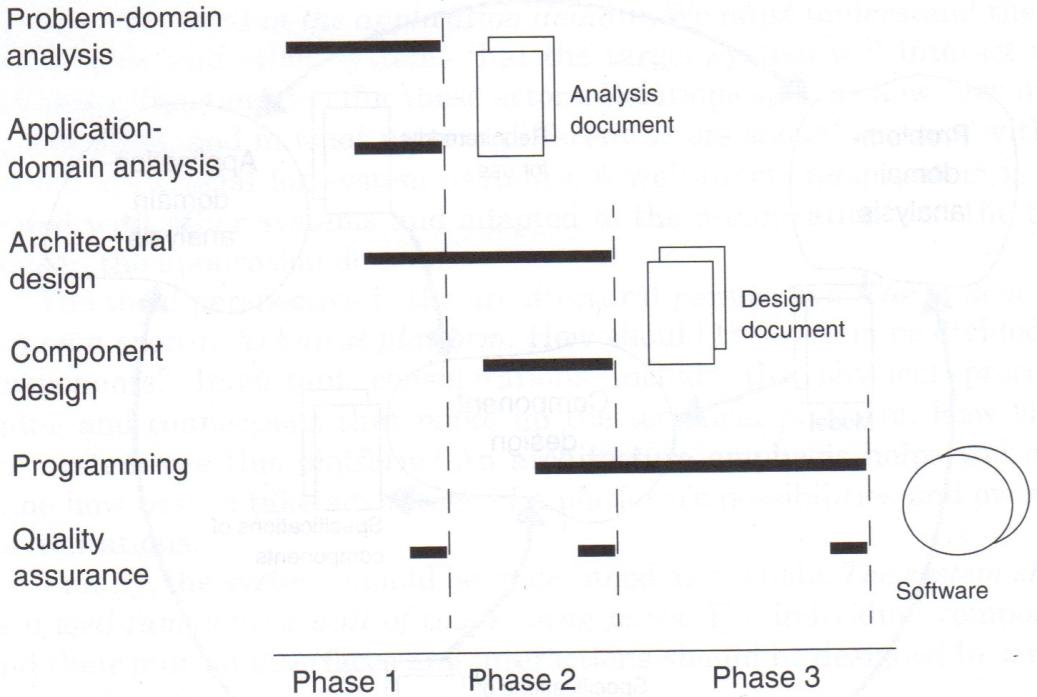
\includegraphics[width=\textwidth]{billeder/SUModel1.jpg}
		\caption{Traditional-top-down approach \citep[p.~16]{Rod-Aalborg}}
		\label{fig:SUModel1}
	\end{subfigure}
	\quad
	\begin{subfigure}[b]{0.48\textwidth}
		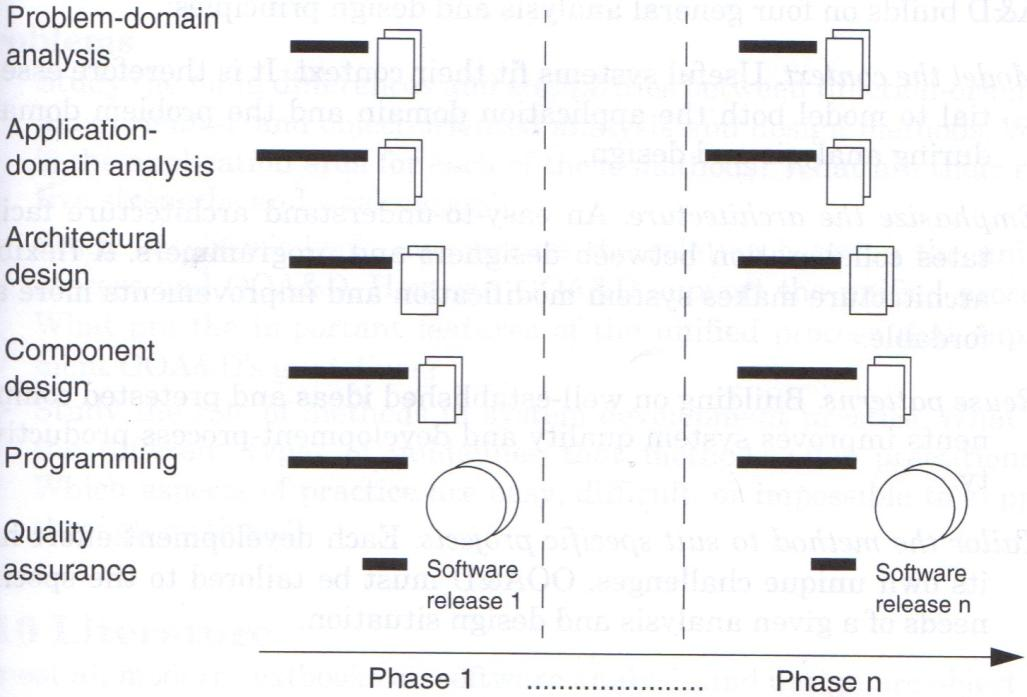
\includegraphics[width=0.9\textwidth]{billeder/SUModel2.jpg}
		\caption{Use-case driven, arcitecture-centric approach \citep[p.~17]{Rod-Aalborg}}
		\label{fig:SUModel2}
	\end{subfigure}
	\caption{Model based on the OOA\&D method}\label{fig:SUModels}
\end{figure}
%\todo[inline]{Lu: specificer hvad vores model er. Vi er nødt til at være meget tydelig med præcis hvilken kombination vi benytter. Benyt figurer og tabeller!!! (evt. for hver sektion)}

\subsection{Using iterative life cycle in the project}
% Henrik: Maaske "Ipsen" i stedet for "specific user's"? :-)
%Anna svar: Kan personligt bedre li denne formulering, da det ikk ekun er Ipsen men også JBJ men kkun med Ipsen som kontakt person. Dog hvis vi gerne vil have den ændret står der et forslag i det udkommenterede lige nedenfor.
%Throughout the project it is intended to design a system iteratively with Ipsen's and JBJ's needs and wants integrated into the designs and tests. 
Throughout the project it is intended to design a system iteratively with a specific user’s needs and wants integrated into the designs and tests. 
The basic idea of the workflow in this process is a a mix of the models pictured in \cref{fig:SUModels}, where most of the basic activities is considered in each iteration, ending with some new notes, thoughts or models and analysis' as seen in \cref{fig:SUModel2}.
The elements of the model in \cref{fig:SUModel1} comes forth in the fact that not every basic activity is considered in every iteration. And some of the activities is finished or considered closed before reaching the last iteration.

As for the main flow in the project it follows the model in \cref{fig:DEBModel}. Where each iteration first tries to understand the current problem then evaluate either in the team or with Ipsen, where from the analysis is developed or reevaluated and a prototype is designed or further developed.
This finally ends the iterations in an interview or usability test, from which the data gathered is used in the next iterative flow.

A clear example of how the system is developed iterativly is furthermore, how the prototype from the end of the first iteration is further developed and added more functionality at each iteration until it is considered finished.
Hereby the final system is not developed in one go as with the waterfall model, \cref{sec:WaterfallModel},  but instead evolved with each iteration.

In the following sections each iteration will be presented, with a comparison to the aforementioned models.
The sections will also contain a mention of the most important changes throughout the specific iterations. 

According to Sharp, Rogers and Preece ''Most projects start with establishing requirements'' \citep[p.~333]{InteractionDesign}. 
It is from this first activity that it is possible to go into the designing and further analysis.
As \cref{sec:Iteration1} will reflect this was also the true starting point of the first iteration.
This is also where the development of \textit{OBHandbooks} started.
